\chapter{Space Colonization Algorithmus} \label{ch:SCA}

Es werden die benötigten Eingaben und der Ablauf des Space Colonization Algorithmus behandelt. Die Prozedur zur Generierung von Baumstrukturen wird vorgestellt und die implementierten Erweiterungen des ursprünglichen Algorithmus werden erläutert.

\section{Ursprung}
Der vorgestellte Space Colonization Algorithmus wurde ursprünglich zur Modellierung und Visualisierung von Blattvenen entwickelt und basiert auf der Wirkung des Pflanzenhormons Auxin. Dieser Hormonstoff entsteht im Blatt und wird von bereits existierenden Blattvenen angezogen, der resultierende Hormonstrom führt zur Bildung von neuen Venen im Blatt. Die Simulation dieses Vorgangs führt zu realitätsnahen Venenmustern. \cite[S.3]{LeafVenation:05}

Mithilfe einer Erweiterung in den dreidimensionalen Raum und Nachbearbeitung der Resultate kann eine Vielfalt von Baum- und Strauchstrukturen generiert werden. \cite[S.2]{SpaceColonizationAlgorithm:07}

\section{Aufbau}

Der Algorithmus verarbeitet eine Menge von Einflusspunkten $S$ und baut darauf basierend einen Baum $G = \langle V,E \rangle$ auf. 

Der Algorithmus benötigt die folgenden Eingaben:

\begin{description}[labelindent]
	\item[\boldmath$d_i$] Der Einflussradius. Einflusspunkte prägen den Aufbau des Baums nur, wenn sich Knotenpunkte innerhalb dieses Radius befinden. \cite[S.3]{SpaceColonizationAlgorithm:07}\\
	
	\item[\boldmath$d_k$] Der Minimalradius. Befindet sich ein Knotenpunkt innerhalb des Minimalradius um einen Einflusspunkt, wird dieser aus der Menge der Einflusspunkte $S$ entfernt. \cite[S.3]{SpaceColonizationAlgorithm:07}\\
	
	\item[\boldmath$D$] Die Schrittweite. Jeder neu generierte Knotenpunkt wird in diesem Abstand zu seinem Vorgänger positioniert. \cite[S.3]{SpaceColonizationAlgorithm:07} \\
	
	\item[\boldmath$\overrightarrow{T}$] Der Tropismusvektor. \cite[S.3]{SpaceColonizationAlgorithm:07}

\end{description}

\section{Ablauf}
\label{sec:SCA_Ablauf}
Zu Beginn des Algorithmus werden $N$ Einflusspunkte in einem vorgegebenen Bereich generiert. Dieser Einflussbereich signalisiert die Verfügbarkeit von Raum, in dem die Baumstruktur entstehen kann.  \cite[S.3]{SpaceColonizationAlgorithm:07}

Daraufhin wird der Baum iterativ aufgebaut und durchläuft in jeder Iteration die folgenden Schritte: 

\begin{description}[labelindent]
	\item[\boldmath$1.$] Für jeden Einflusspunkt in $S$ wird der am nächsten liegende Knotenpunkt $v\in V$ bestimmt. Befindet sich $v$ innerhalb des Einflussradius $d_i$ eines Einflusspunktes, wird der Knotenpunkt einer zugeordneten Menge $S(v)$ hinzugefügt. $S(v)$ beinhaltet somit alle Einflusspunkte, die einen Einfluss auf den Knotenpunkt ausüben. \cite[S.3]{SpaceColonizationAlgorithm:07} \label{alg:SCA_1}\\
	
	\item[\boldmath$2.$] Befinden sich Elemente in $S(v)$, wird ein neuer Knotenpunkt $v_n$ den Nachfolgern von $v$ hinzugefügt und $v$ als Vorgänger von $v_n$ eingetragen.  Alle Punkte in $S(v)$ beeinflussen $v_n$ in gleichem Maße, die neue Position $\overrightarrow{p_{v_n}}$ des Knotenpunkts berechnet sich somit wie folgt:
	
	\begin{equation}
	\begin{array}{ll}
	\overrightarrow{p_{v_n}} & = \overrightarrow{p_v} + D * \overrightarrow{n_{T}}
	\end{array}
	\end{equation} 
	
	\begin{equation}
	\begin{array}{ll}
	\text{  mit  } \overrightarrow{n_{T}} & = \dfrac{\overrightarrow{n} + \overrightarrow{T} }{\lVert\overrightarrow{n} + \overrightarrow{T}\rVert}  
	\end{array}
	\end{equation} 
	
	\begin{equation}
	\begin{array}{ll}
	\text{ und }  \overrightarrow{n} = \sum\limits_{s \in S(v)}\dfrac{\overrightarrow{p_s} - \overrightarrow{p_v}}{\lVert \overrightarrow{p_s} - \overrightarrow{p_v} \rVert}
	\end{array}
	\end{equation}	
	\cite[S.3]{SpaceColonizationAlgorithm:07} \label{alg:SCA_2}\\
	
	\item[\boldmath$3.$] Für jeden Einflusspunkt wird überprüft, ob sich ein Knotenpunkt innerhalb des Minimalradius $d_k$ befindet. Existiert ein solcher Knotenpunkt, wird der Einflusspunkt aus der Menge der Einflusspunkte $S$ entfernt. \cite[S.3]{SpaceColonizationAlgorithm:07} \label{alg:SCA_3}
\end{description}

Diese Schritte werden solange ausgeführt, bis alle Einflusspunkte entfernt wurden, sich kein Knotenpunkt im Einflussradius eines Einflusspunktes befindet oder bis eine vorgegebene Maximalanzahl von Iterationen durchgeführt wurde. \cite[S.2]{SpaceColonizationAlgorithm:07} Abbildung \ref{fig:SCA_Basic} zeigt eine beispielhafte Anwendung des Algorithmus.

\begin{figure} [hbtp]
	\centering
	\begin{subfigure}[t]{.31\textwidth}
		\centering
		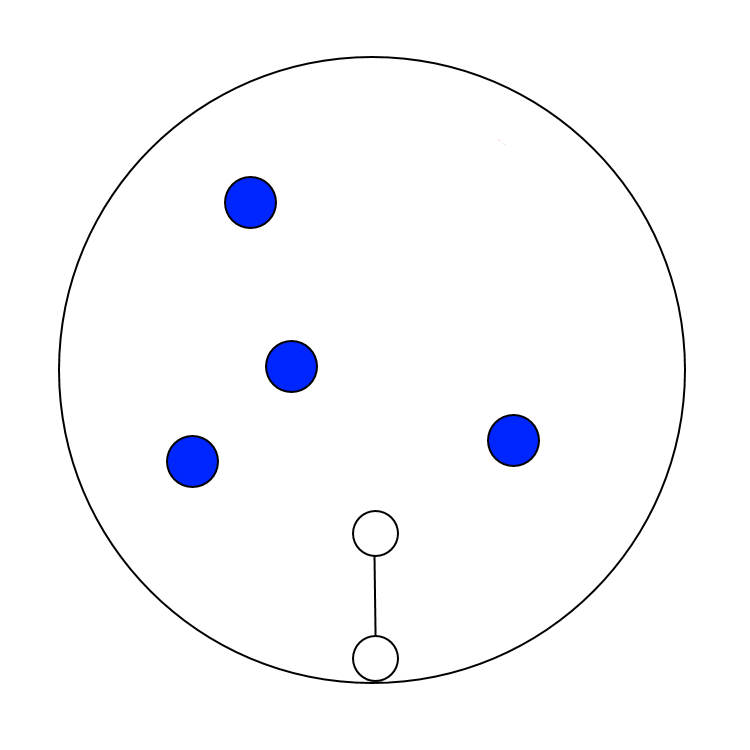
\includegraphics[width=\linewidth]{images/SCA_Basic1.png}
		\caption{ Ausgangssituation. }
		\label{subfig:SCA_Basic1}
	\end{subfigure}
	\hspace{.01\textwidth}
	\begin{subfigure}[t]{.31\textwidth}
		\centering
		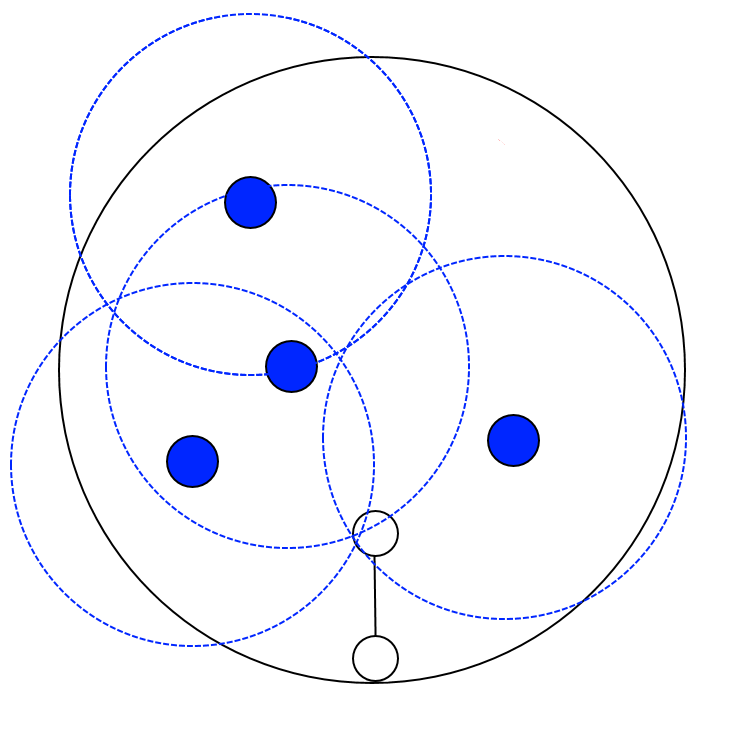
\includegraphics[width=\linewidth]{images/SCA_Basic2.png}
		\caption{Schritt 1: Blaue Kreise entsprechen dem Einflussradius.}
		\label{subfig:SCA_Basic2}
	\end{subfigure}
	\hspace{.01\textwidth}
	\begin{subfigure}[t]{.31\textwidth}
		\centering
		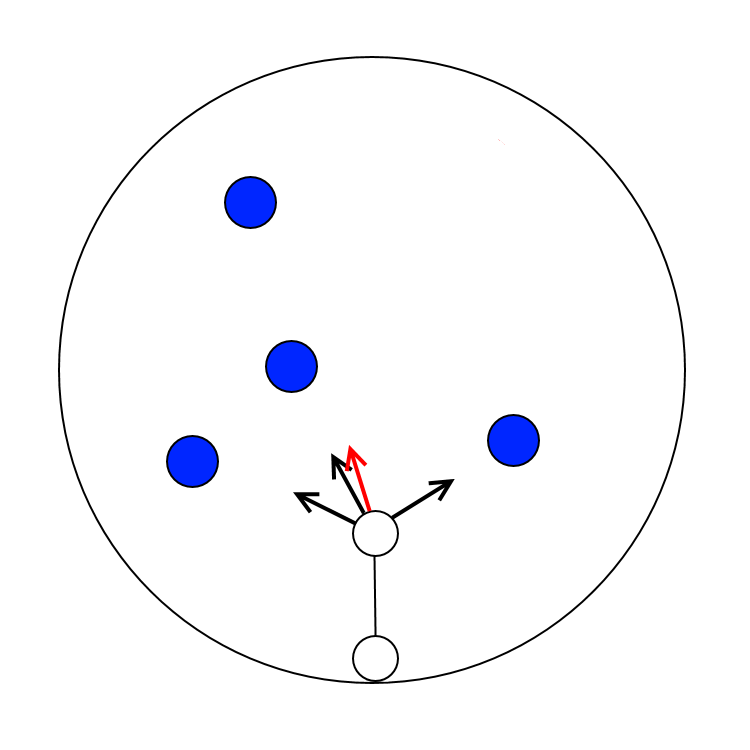
\includegraphics[width=\linewidth]{images/SCA_Basic3.png}
		\caption{Schritt 2: Bestimmung von $\overrightarrow{n_T}$ (roter Pfeil) ohne Einbeziehung von $\overrightarrow{T}$.}
		\label{subfig:SCA_Basic3}
	\end{subfigure}

	\begin{subfigure}[t]{.31\textwidth}
		\centering
		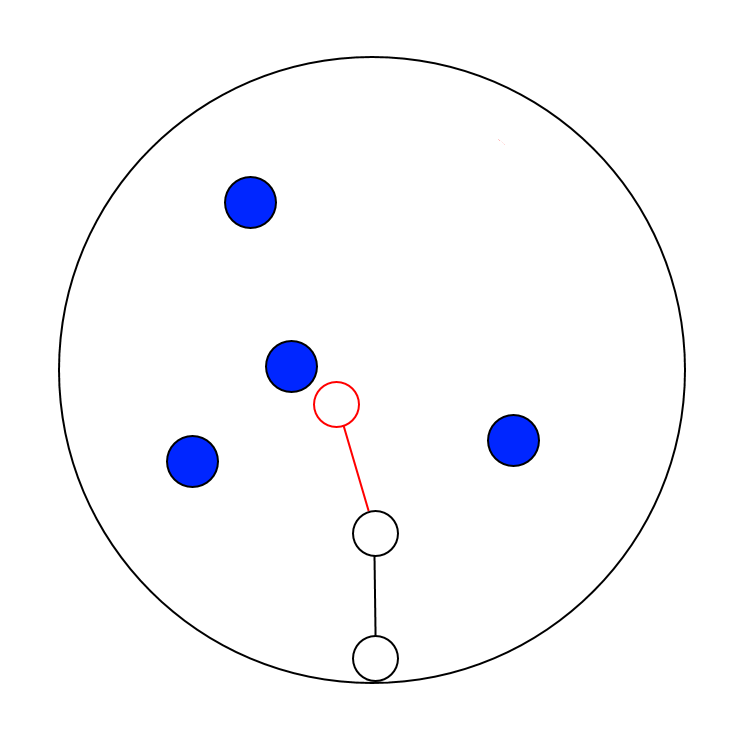
\includegraphics[width=\linewidth]{images/SCA_Basic4.png}
		\caption{Schritt 2: Platzierung des neuen Knotenpunkts.}
		\label{subfig:SCA_Basic4}
	\end{subfigure}
	\hspace{.01\textwidth}
	\begin{subfigure}[t]{.31\textwidth}
		\centering
		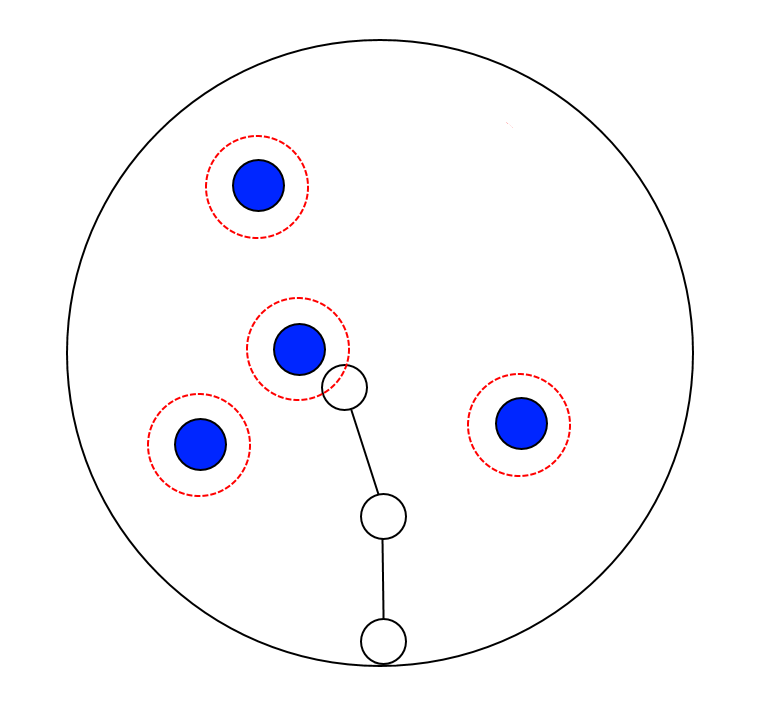
\includegraphics[width=\linewidth]{images/SCA_Basic5.png}
		\caption{Schritt 3: Rote Kreise entsprechen dem Minimalradius.}
		\label{subfig:SCA_Basic5}
	\end{subfigure}
	\hspace{.01\textwidth}
	\begin{subfigure}[t]{.31\textwidth}
		\centering
		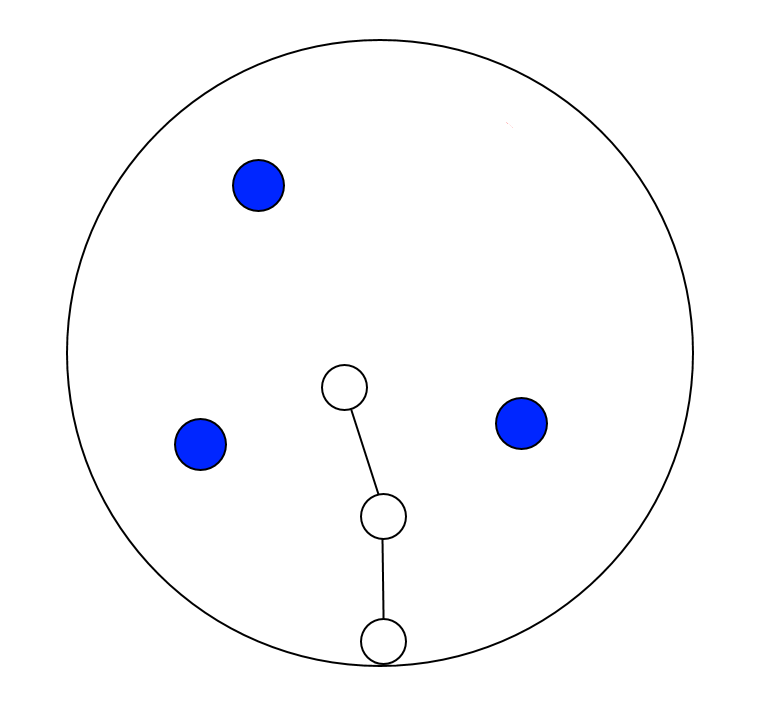
\includegraphics[width=\linewidth]{images/SCA_Basic6.png}
		\caption{Ausgangssituation der nächsten Iteration.}
		\label{subfig:SCA_Basic6}
	\end{subfigure}

	\begin{subfigure}[t]{.31\textwidth}
		\centering
		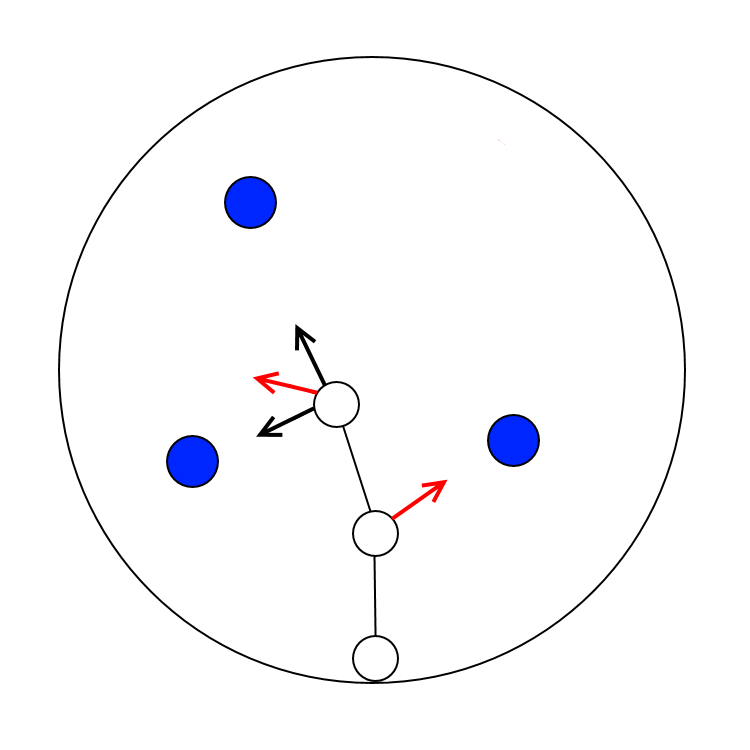
\includegraphics[width=\linewidth]{images/SCA_Basic7.png}
		\caption{Einflusspunkte beeinflussen unterschiedliche Knotenpunkte.}
		\label{subfig:SCA_Basic7}
	\end{subfigure}
	\hspace{.01\textwidth}
	\begin{subfigure}[t]{.31\textwidth}
		\centering
		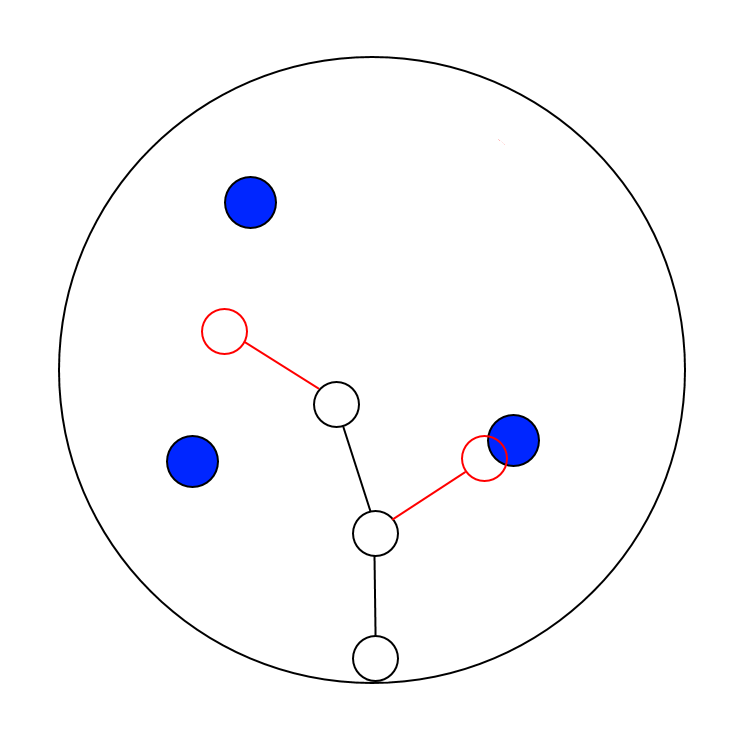
\includegraphics[width=\linewidth]{images/SCA_Basic8.png}
		\caption{Eine Verzweigung entsteht.}
		\label{subfig:SCA_Basic8}
	\end{subfigure}
	\caption{Beispielhafte Anwendung des Space Colonization Algorithmus. Blaue Punkte entsprechen Einflusspunkten, weiße Punkte entsprechen Knotenpunkten. Der unterste Knotenpunkt stellt die Wurzel dar. Eigene Abbildungen auf Grundlage von \cite[Abb. 2]{SpaceColonizationAlgorithm:07}.}\label{fig:SCA_Basic}
	
\end{figure}


\section{Generierung von Baumstrukturen}
\label{sec:GenerierungBaumstrukturen}
Der Space Colonization Algorithmus liefert einen Baum, der Knotenpunkte enthält, welche Positionen im dreidimensionalen Raum entsprechen. Um diese Knotenpunkte in Form von baumähnlichen Strukturen zu visualisieren, wird die Prozedur erweitert. Der Aufbau der Baumstruktur läuft wie folgt ab:

\begin{description}[labelindent]
	\item[\boldmath$1.$] Der Einflussbereich wird mit der vorgegeben Anzahl von Einflusspunkten gefüllt. \cite[S.2]{SpaceColonizationAlgorithm:07} \\

	\item[\boldmath$2.$] Der Baum wird, wie in Abschnitt \ref{sec:SCA_Ablauf} beschrieben, iterativ generiert. \cite[S.2]{SpaceColonizationAlgorithm:07} \\

	\item[\boldmath$3.$] Die Nachfolger jedes Knotenpunkts werden einander angenähert, um eine Verringerung der Abzweigungswinkel zwischen den verbindenden Kanten zu erreichen. Dies führt zu einer insgesamt realistischeren Baumstruktur. \cite[S.2]{SpaceColonizationAlgorithm:07} \\
	
	\item[\boldmath$4.$] Die Kanten, welche die Knotenpunkte verbinden, werden mithilfe von Zylindern visualisiert, um die Aststruktur eines biologischen Baumes zu simulieren. \cite[S.2]{SpaceColonizationAlgorithm:07} 
	
\end{description}

Die von Runions u.a. \cite{SpaceColonizationAlgorithm:07} vorgeschlagene Kurven-Unterteilung \cite[S.2]{SpaceColonizationAlgorithm:07} wurde in dieser Arbeit nicht behandelt, da durch Angabe der Schrittweite $D$ eine ausreichende, visuelle Qualität erzielt wurde.

Abbildung \ref{fig:SCA_Extended} zeigt die Modellierung einer zweidimensionalen Baumstruktur.

\paragraph{Verringerung der Abzweigungswinkel} \label{par:VerringerungAbzweigungswinkel}

Die $m$ Nachfolger $v_{1} ... v_{m}$ eines Knotens $v$ werden wie folgt einander angenähert:
\begin{equation}
\overrightarrow{m} = \overrightarrow{p_v} + \dfrac{\sum_{i=0}^{m} (\overrightarrow{p_{v_i}} - \overrightarrow{p_v})}{m}
\end{equation}

wobei $\overrightarrow{m}$ dem arithmetischen Mittelpunkt der Nachfolger entspricht. Die Positionen der Nachfolger werden nun wie folgt dem Mittelpunkt angenähert:

\begin{equation}
\overrightarrow{p_{v_i}} = \overrightarrow{p_{v_i}} + \dfrac{\overrightarrow{m} -\overrightarrow{p_{v_i}}}{2}
\end{equation}

\cite[S.2]{SpaceColonizationAlgorithm:07}


\paragraph{Berechnung der Zylinderbreiten}

Die Berechnung der Zylinderbreiten erfolgt anhand von Murrays Regel, welche besagt, dass der Radius $r$ eines Astes auf Grundlage der Radien $r_{n_1}...r_{n_m}$ der nachfolgenden, von ihm abzweigenden Äste wie folgt berechnet werden kann: 

\begin{equation}
\begin{array}{ll}
r^g & = r_{n_1}^g + r_{n_2}^g + ... + r_{n_m}^g 
\end{array}
\label{eq:Radiusberechnung}
\end{equation} 

Diese Berechnung kann rekursiv auf dem Baum ausgeführt werden, indem für jeden Knotenpunkt der Radius aus den Radien seiner Nachfolger berechnet wird. Besitzt ein Knotenpunkt keine Nachfolger, wird ein festgelegter Radius $r_0$ zurückgegeben. Der Wert $g$ kann frei gewählt werden. \cite[S.5]{LeafVenation:05}

\begin{figure} [htbp]
	\centering
	\begin{subfigure}[t]{.4\textwidth}
		\centering
		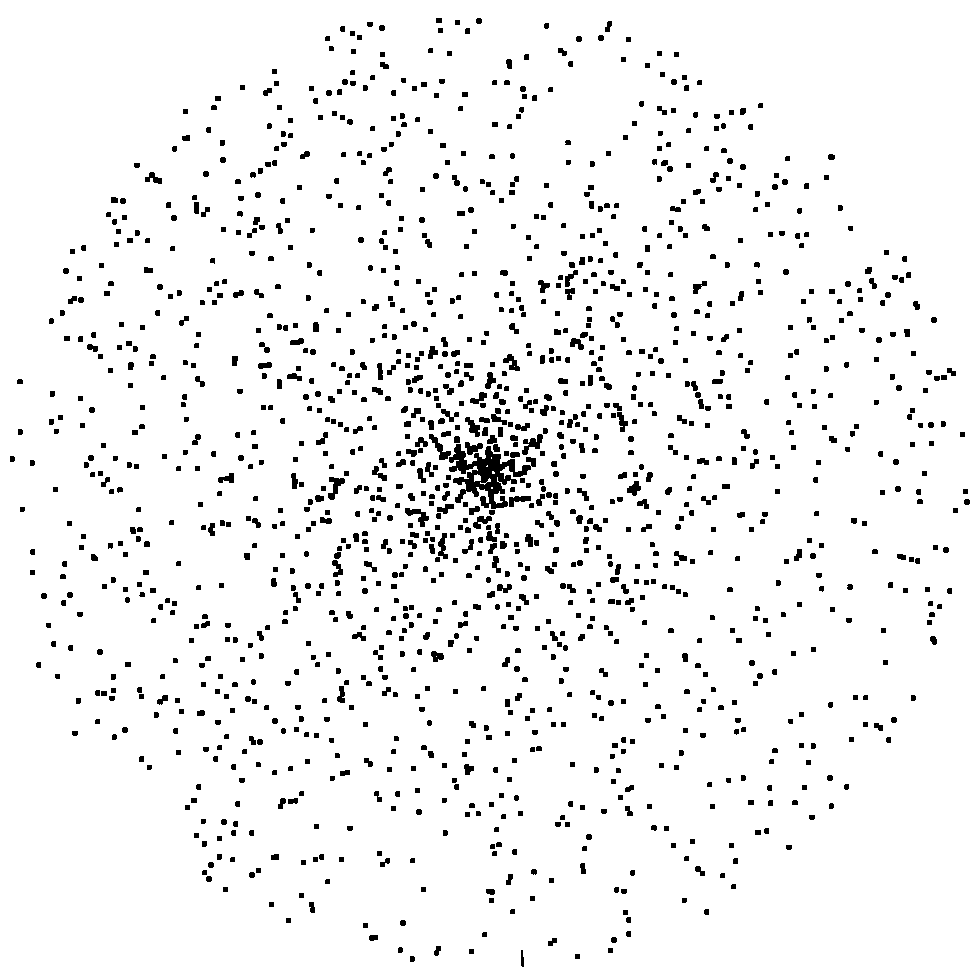
\includegraphics[width=\linewidth]{images/SCA_Extended1.png}
		\caption{$N=2000$ Einflusspunkte, zufällig in einem Ring mit dem Radius $r = 500$ verteilt.}
		\label{subfig:SCA_Extended1}
	\end{subfigure}
	\hspace{.1\textwidth}
	\begin{subfigure}[t]{.4\textwidth}
		\centering
		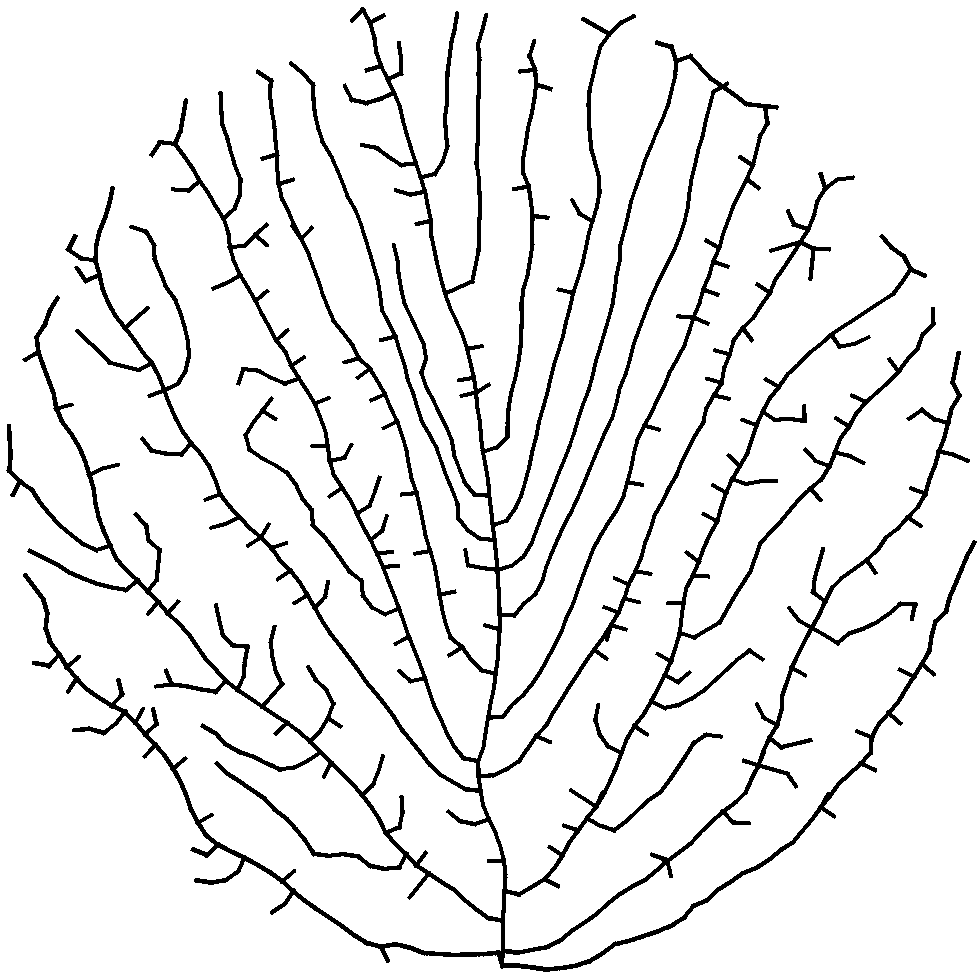
\includegraphics[width=\linewidth]{images/SCA_Extended2.png}
		\caption{Ergebnis des Space Colonization Algorithmus mit einem Einflussradius $d_i = 100$, Minimalradius $d_k = 20$, Schritteweite $D = 15$ und $\overrightarrow{T} = \overrightarrow{0}$.}
		\label{subfig:SCA_Extended2}
	\end{subfigure}
	\begin{subfigure}[t]{.4\textwidth}
		\centering
		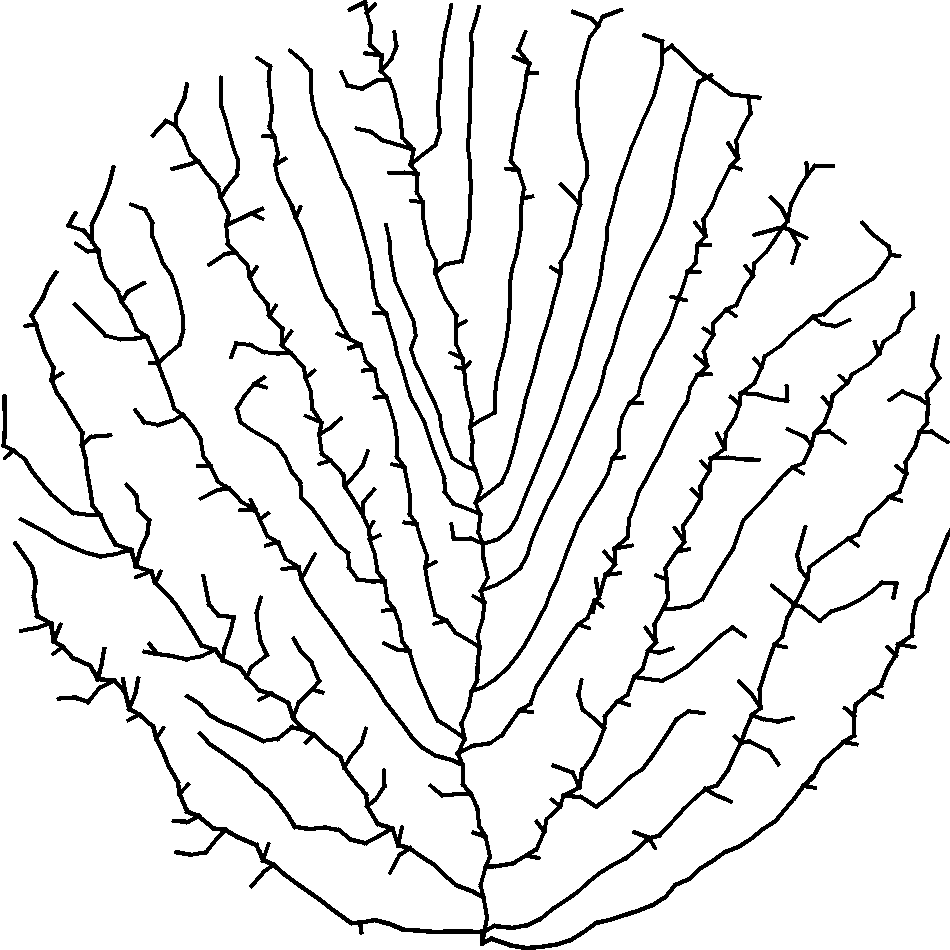
\includegraphics[width=\linewidth]{images/SCA_Extended3.png}
		\caption{Verringerung der Abzweigungswinkel.}
		\label{subfig:SCA_Extended3}
	\end{subfigure}
	\hspace{.1\textwidth}
	\begin{subfigure}[t]{.4\textwidth}
		\centering
		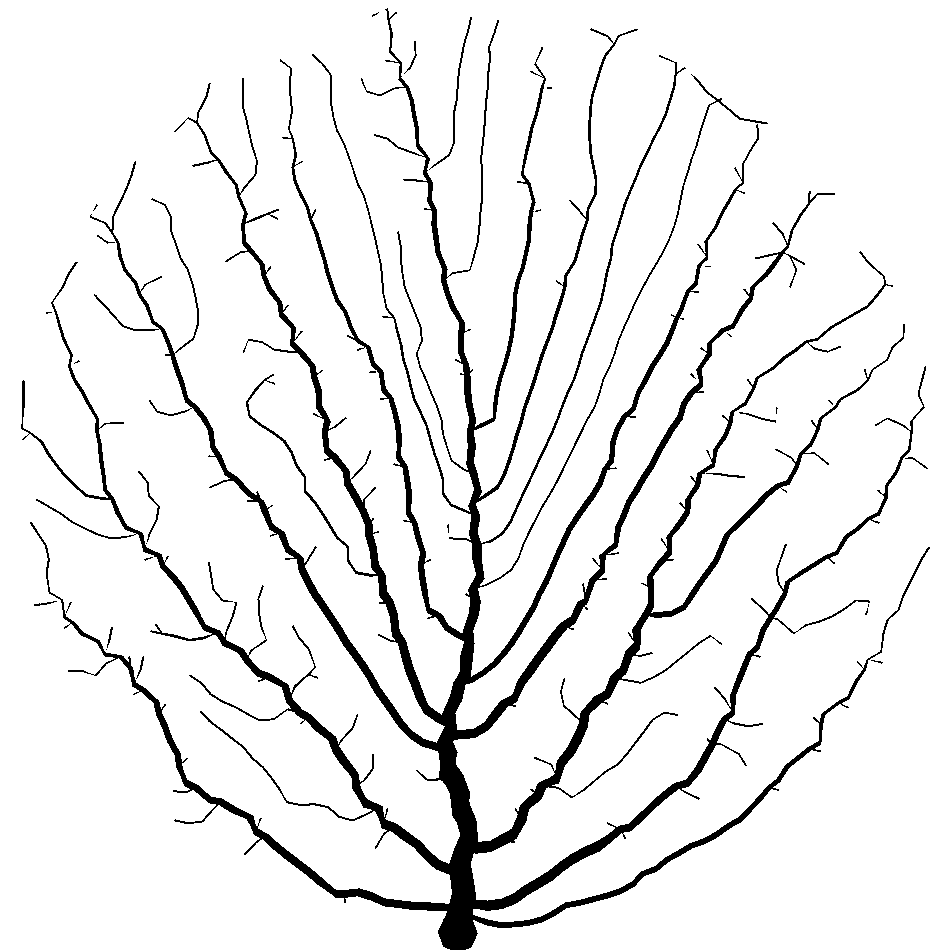
\includegraphics[width=\linewidth]{images/SCA_Extended4.png}
		\caption{Modellierung des Ergebnis mithilfe von Zylindern mit $r_0 = 1$ und $g=2$.}
		\label{subfig:SCA_Extended4}
	\end{subfigure}
	\caption{Modellierung einer zweidimensionalen Baumstruktur entsprechend der in Abschnitt \ref{sec:GenerierungBaumstrukturen} beschriebenen Schritte. Eigene Abbildungen.}
	\label{fig:SCA_Extended}
\end{figure}

\section{Erweiterungen} \label{sec:SCA_Erweiterungen}

Im Rahmen dieser Arbeit wurden die folgenden Erweiterungen des ursprünglichen Algorithmus entwickelt und implementiert.

\paragraph{Zweigtiefe}

Die Zweigtiefe $Z(v)$ eines Knotens $v \in V$ wird für Erweiterungen des Space Colonization Algorithmus und die Generierung von Modelldaten verwendet. Sie entspricht nicht der Tiefe des Knotens und berechnet sich wie folgt:
\begin{equation}
Z(v)= \begin{cases}
0 & \text{falls v die Wurzel ist} \\
Z(v') & \text{falls v' genau einen Nachfolger besitzt}\\
1 + Z(v') & \text{sonst}
\end{cases} 
\end{equation}
wobei $v'$ den Vorgänger des Knotens $v$ darstellt. Die Zweigtiefe wird direkt nach der Erstellung des Knotens berechnet und daraufhin nicht verändert. Ein Beispiel für die Bestimmung der Zweigtiefe wird in Abbildung \ref{fig:SCA_Zweigtiefe} gezeigt.

Der von Prusinkiewicz u.a. \cite{ABOP:04} beschriebene Begriff von axialen Bäumen \cite[S.21]{ABOP:04} und die zugehörige Bestimmung der Achsentiefe unterscheidet sich von der Berechnung der Zweigtiefe. Knoten können dieselbe Zweigtiefe besitzen, selbst wenn die Verbindung ihrer Positionen keine gerade Linie bildet.

\begin{figure} [hbtp]
	\centering
	\begin{subfigure}[t]{.31\textwidth}
		\centering
		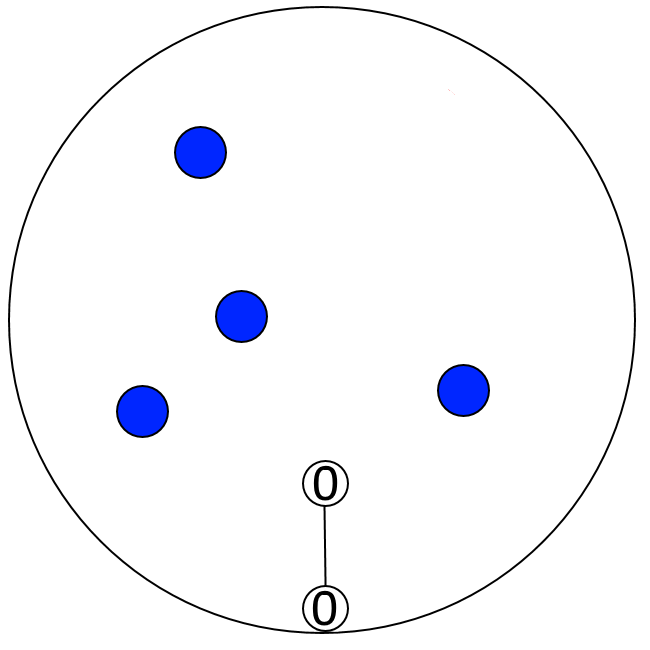
\includegraphics[width=\linewidth]{images/SCA_Zweigtiefe1.png}
		\caption{Ausgangssituation.}
		\label{subfig:SCA_Zweigtiefe1}
	\end{subfigure}
	\hspace{.01\textwidth}
	\begin{subfigure}[t]{.31\textwidth}
		\centering
		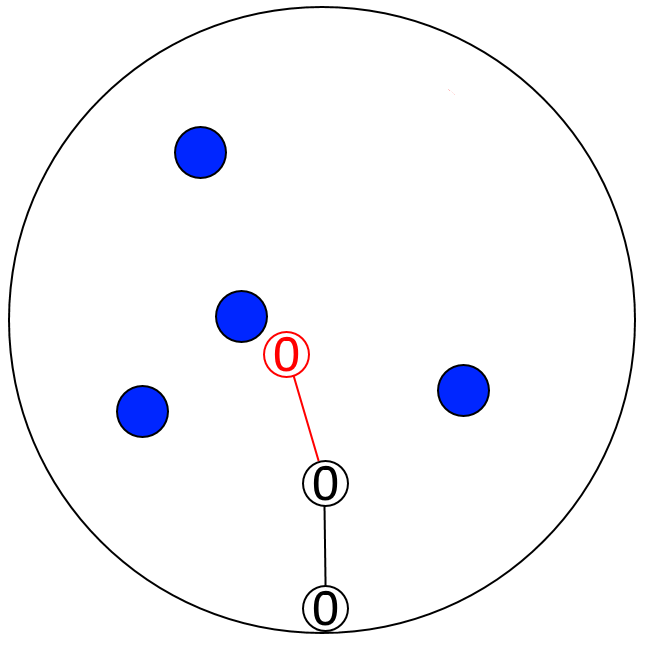
\includegraphics[width=\linewidth]{images/SCA_Zweigtiefe2.png}
		\caption{Der Vorgänger des neuen Knotens besitzt genau einen Nachfolger.}
		\label{subfig:SCA_Zweigtiefe2}
	\end{subfigure}
	\hspace{.01\textwidth}
	\begin{subfigure}[t]{.31\textwidth}
		\centering
		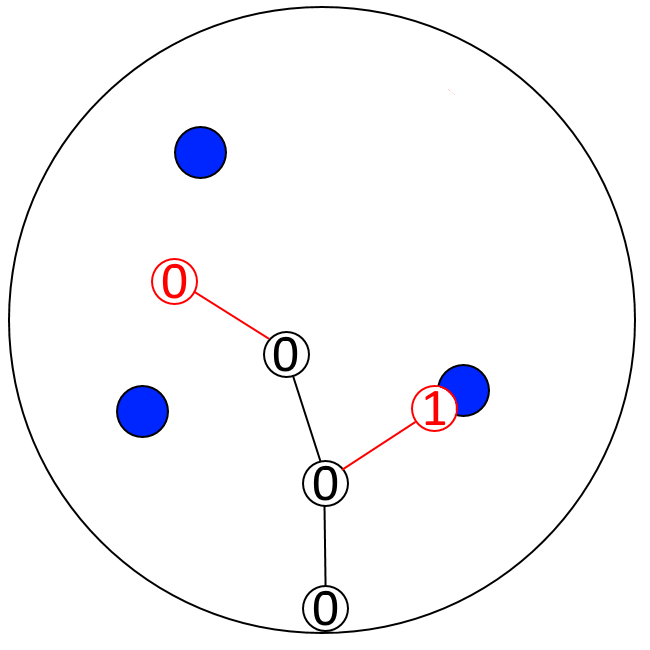
\includegraphics[width=\linewidth]{images/SCA_Zweigtiefe3.png}
		\caption{Die Zweigtiefe des rechten neuen Knotens ist um $1$ größer als der seines Vorgängers, da dieser mehr als einen Nachfolger besitzt.}
		\label{subfig:SCA_Zweigtiefe3}
	\end{subfigure}
	\caption{Darstellung der Zweigtiefen von Knotenpunkten aus Abbildung \ref{fig:SCA_Basic}. }
	\label{fig:SCA_Zweigtiefe}
\end{figure}

\paragraph{Zusätzliche Bedingungen}

Um die vom Space Colonization Algorithmus generierte Baumstruktur besser kontrollieren zu können, wurden zusätzliche Bedingungen zum Ablauf des Algorithmus hinzugefügt:
\begin{description}[labelindent]
	\item[\boldmath$max_{grad}$] Der maximale Grad der Knotenpunkte im Baum. Bevor ein neuer Knotenpunkt $v_n$ als Nachfolger eines Knotenpunkts $v$ erstellt wird, wird die Anzahl der Nachfolger von $v$ überprüft. Entspricht diese $max_{grad}$, wird der Knotenpunkt $v_n$ nicht erstellt.\\
	
	\item[\boldmath$max_{Z}$] Die maximale Zweigtiefe eines Knotens. Bevor ein neuer Knotenpunkt $v_n$ als Nachfolger eines Knotenpunkts $v$ erstellt wird, wird seine Zweigtiefe $Z(v_n)$ berechnet. Übersteigt diese $max_{Z}$, wird der Knotenpunkt $v_n$ nicht erstellt.\\
	
	\item[\boldmath$max_{NG}$] Die maximale Anzahl von Iterationen, in welchen einem Knotenpunkt kein neuer Nachfolger hinzugefügt wurde.\footnote{$NG$ steht für \glqq No Grow\grqq{} oder \glqq Did not grow\grqq, englisch für \glqq kein Wachstum\grqq.} Hat ein Knoten diesen Wert erreicht, wird er in Schritt 1 des Algorithmus \ref{alg:SCA_1} nicht weiter darauf untersucht, ob er sich innerhalb des Einflussradius eines Einflusspunktes befindet. Der Wert von $max_{NG}$ eines Knotenpunkts wird auf $0$ zurückgesetzt, falls diesem ein neuer Nachfolger hinzugefügt wurde.
	
	Durch die vorsichtige Wahl von $max_{NG}$ können Positionsvergleiche vermieden werden ohne den resultierenden Baum visuell erkennbar zu verändern.
\end{description}

\paragraph{Gewichtetes Wachstum}

Gewichtetes Wachstum ist eine Möglichkeit die Schrittweite $D$ in Abhängigkeit von der Zweigtiefe zu erhöhen. Befindet sich ein Knotenpunkt auf der Zweigtiefe $0$, werden neu hinzugefügte Nachfolger im Abstand von $2 * D$ positioniert, befindet er sich auf der maximalen Zweigtiefe, werden neu hinzugefügte Nachfolger im Abstand von $D$ positioniert. Zwischen diesen beiden Zweigtiefen wird die Schrittweite linear interpoliert.

\paragraph{Kurvenreduktion} \label{par:Kurvenreduktion}
 
Kurvenreduktion in Abhängigkeit des Abzweigungswinkels ermöglicht es die Baumstruktur mithilfe einer verringerten Datenmenge darzustellen. Besitzt ein Knoten $v$ genau einen Nachfolger $v_n$ und einen Vorgänger $v'$, werden die zwei Richtungsvektoren zwischen $v'$ und $v$ sowie $v$ und $v_n$ berechnet:
\begin{equation}
\overrightarrow{R_1} = \dfrac{\overrightarrow{p_v} - \overrightarrow{p_{v'}}}{\lVert\overrightarrow{p_v} - \overrightarrow{p_{v'}} \rVert} \text{ und } \overrightarrow{R_2} = \dfrac{\overrightarrow{p_{v_n}} - \overrightarrow{p_{v}}}{\lVert \overrightarrow{p_{v_n}} - \overrightarrow{p_{v}} \rVert}
\end{equation}

Übersteigt das Skalarprodukt $\langle \overrightarrow{R_1}, \overrightarrow{R_2} \rangle$ einen festgelegten Maximalwert $max_K$ zwischen $0$ und $1$, wird $v$ aus dem Baum entfernt. $v_n$ wird zum Nachfolger von $v'$ und $v'$ zum Vorgänger von $v_n$. 

Die Kurvenreduktion kann auch auf Bäume angewendet werden, welche wie in Abschnitt \ref{sec:LS_Baumstrukturen} beschrieben durch eine Turtle-Interpretation aufgebaut wurden.